\documentclass[red,10pt]{beamer}
%\setbeamertemplate{theorems}[numbered]
\usetheme{Warsaw}
\usecolortheme{default}
\usepackage{makeidx}
\usepackage[brazil]{babel}
\usepackage[utf8]{inputenc}
\usepackage[T1]{fontenc}
\graphicspath{{./figuras/}}             % caminho das figuras (recomendável)
\usepackage[noend]{algorithmic}
\usepackage{algorithm}
\usepackage{qtree}
\usepackage{graphicx}
\usepackage[caption=false]{subfig}
\uselanguage{portuguese}
\languagepath{portuguese}
\newtheorem{proposition}{Proposição}
\newtheorem{assertion}{Asserção}
\newtheorem{conjecture}{Conjectura}
\deftranslation[to=portuguese]{Theorem}{Teorema}
\deftranslation[to=portuguese]{Definition}{Definição}
\deftranslation[to=portuguese]{Fact}{Fato}
\deftranslation[to=portuguese]{Lemma}{Lema}
\usepackage{enumerate}
\algsetup{indent=2em}
\usepackage{tikz}
\usetikzlibrary{trees}
\algsetup{linenodelimiter=\ }
\floatname{algorithm}{Algoritmo}
\newcommand{\GL}{Gyárfás \& Lehel}

\title{Teoria dos Números e Computação: Uma abordagem utilizando problemas de competições de programação}
%\title{Teoria dos Números e Computação: Uma abordagem utilizando problemas de competições de programação}
\author{Antonio Roberto de Campos Junior \\ {Supervisor: Carlos Eduardo Ferreira } }
\institute{Instituto de Matemática e Estatística\\Universidade de São Paulo}
%\date{}

\begin{document}

\frame{\titlepage}
  
\frame{
	\frametitle{Agenda}
	\tableofcontents[ 
		currentsubsection, 
		hideothersubsections, 
		sectionstyle=show, 
		subsectionstyle=show,
		] 
}

\section{Introdução}

\frame{
	\frametitle{Objetivos}
	\begin{itemize}[<+->]
		\setlength{\itemsep}{5pt}
		\item Estudar tópicos específicos relacionados à Teoria dos Números
		\item Criar um material que mostre a aplicação direta dessa teoria na solução de problemas de competições de programação
		\item Demonstração da teoria e implementação dos algoritmos que resolvem os problemas que serão abordados
	\end{itemize}
}
\setcounter{subfigure}{0}


\frame{
	\frametitle{Motivação}
	\begin{itemize}[<+->]
		\setlength{\itemsep}{5pt}
		\item Experiência nesse tipo de competição
		\item Falta de um bom material didático nesse molde
	\end{itemize}
}
\setcounter{subfigure}{0}


\section {Crivo}
\begin{frame}{\secname}
  \tableofcontents[currentsection,currentsubsection]
\end{frame}
\frame{
\frametitle{Crivo de Erastótenes}
Algoritmo criado pelo matemático \textbf{Erastótenes} (a.C. 285-194 a.C.) para o cálculo de números primos
até um certo valor limite $N$.
O algoritmo mantém uma tabela com $N$ elementos, e para cada primo, começando pelo número $2$, marca na tabelo os números compostos múltiplos desses primos.
Desse modo, ao final do algoritmo, os elementos não marcados são números primos.
\newline

\begin{figure}%[!htb]
    \centering
    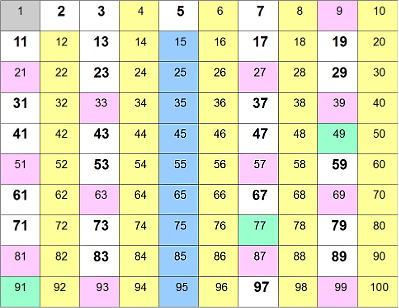
\includegraphics[width=0.3\linewidth]{crivo.jpg}
    \caption{Tabela usado no \textit{Crivo de Erastóteles} com $N=100$.}
\end{figure}
}
\setcounter{subfigure}{0}


\frame{
\frametitle{Pseudocódigo}
\begin{figure}%[!htb]
    \centering
    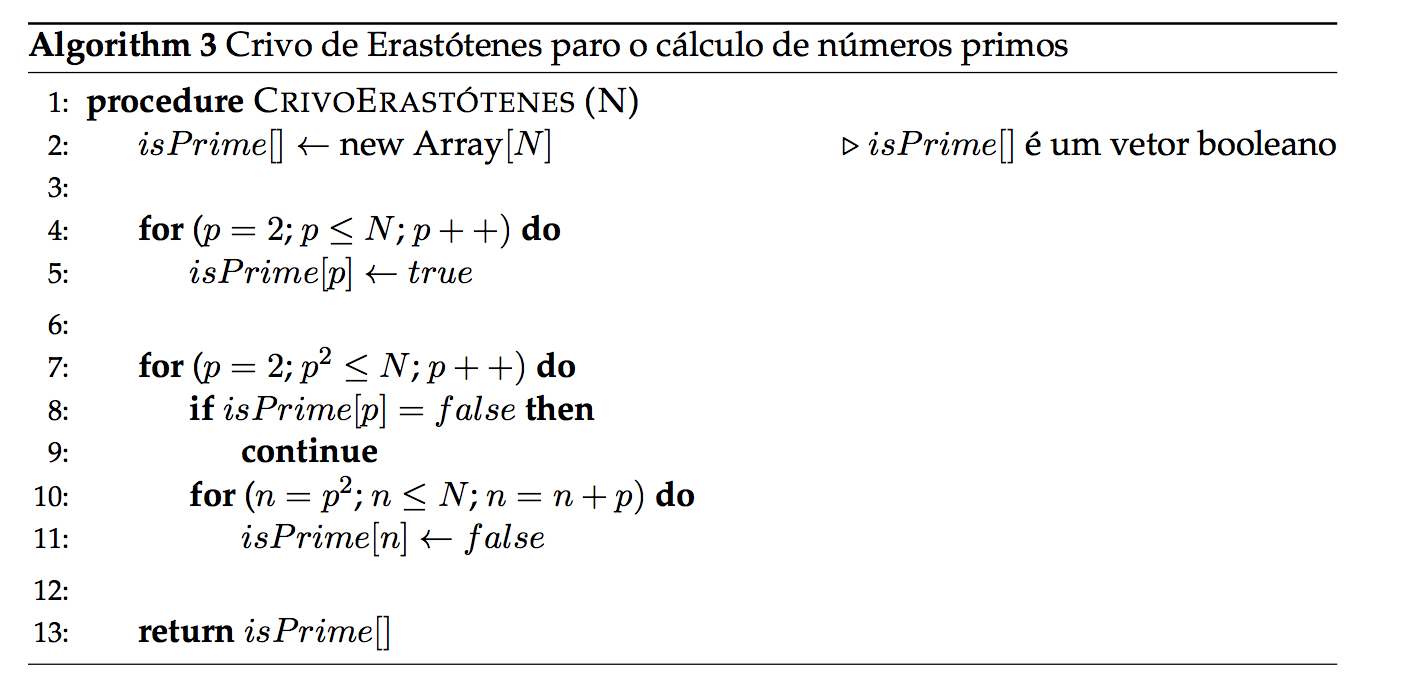
\includegraphics[width=0.8\linewidth]{code.png}
\end{figure}
}
\setcounter{subfigure}{0}





\section {Problema}
\begin{frame}{\secname}
  \tableofcontents[currentsection,currentsubsection]
\end{frame}


\frame{
\frametitle{Problema Exemplo: Goldbach's Conjecture}
\textbf{Link do Problema: }\url{https://uva.onlinejudge.org/index.php?option=onlinejudge&page=show_problem&problem=484}
\newline

\textbf{Resumo: }
É dado um número inteiro $n$ ($6 \leq n < 10^6$). O problema consiste em verificar se $n$ pode ser escrito como a soma de dois números primos ímpares. E em caso positivo dizer quais são esses primos.
}
\setcounter{subfigure}{0}


\frame{
\frametitle{Solução}
Para resolver esse problema basta rodar o \textbf{Crivo de Erastótenes} para $N=n$, e fazer uma varredura linear no vetor $isPrime[]$. Se existir um índice $a$ ($6 \leq a \leq n$) tal que $isPrime[a]$ é $true$ e $isPrime[n-a]$ também é $true$, então o problema acima tem solução.
\newline

\begin{figure}%[!htb]
    \centering
    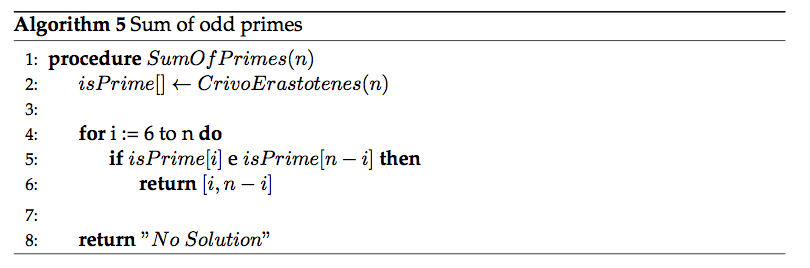
\includegraphics[width=0.8\linewidth]{solution.png}
    \caption{Pseudocódigo da solução acima.}
\end{figure}
}
\setcounter{subfigure}{0}


\section{Curiosidades}

\begin{frame}{\secname}
  \tableofcontents[currentsection,currentsubsection]
\end{frame}

\frame {
	\frametitle{Curiosidades da ACM-ICPC}

Nos últimos anos a ACM-ICPC teve um crescimento significativo. Se compararmos
o número de competidores, temos que de 1997 (ano em que começou o patrocinio
da IBM) até 2014 houve um aumento maior que $1500\%$, totalizando 38160
competidores de 2534 universidades em 101 países ao redor do mundo.

\begin{figure}%[!htb]
    %\centering
    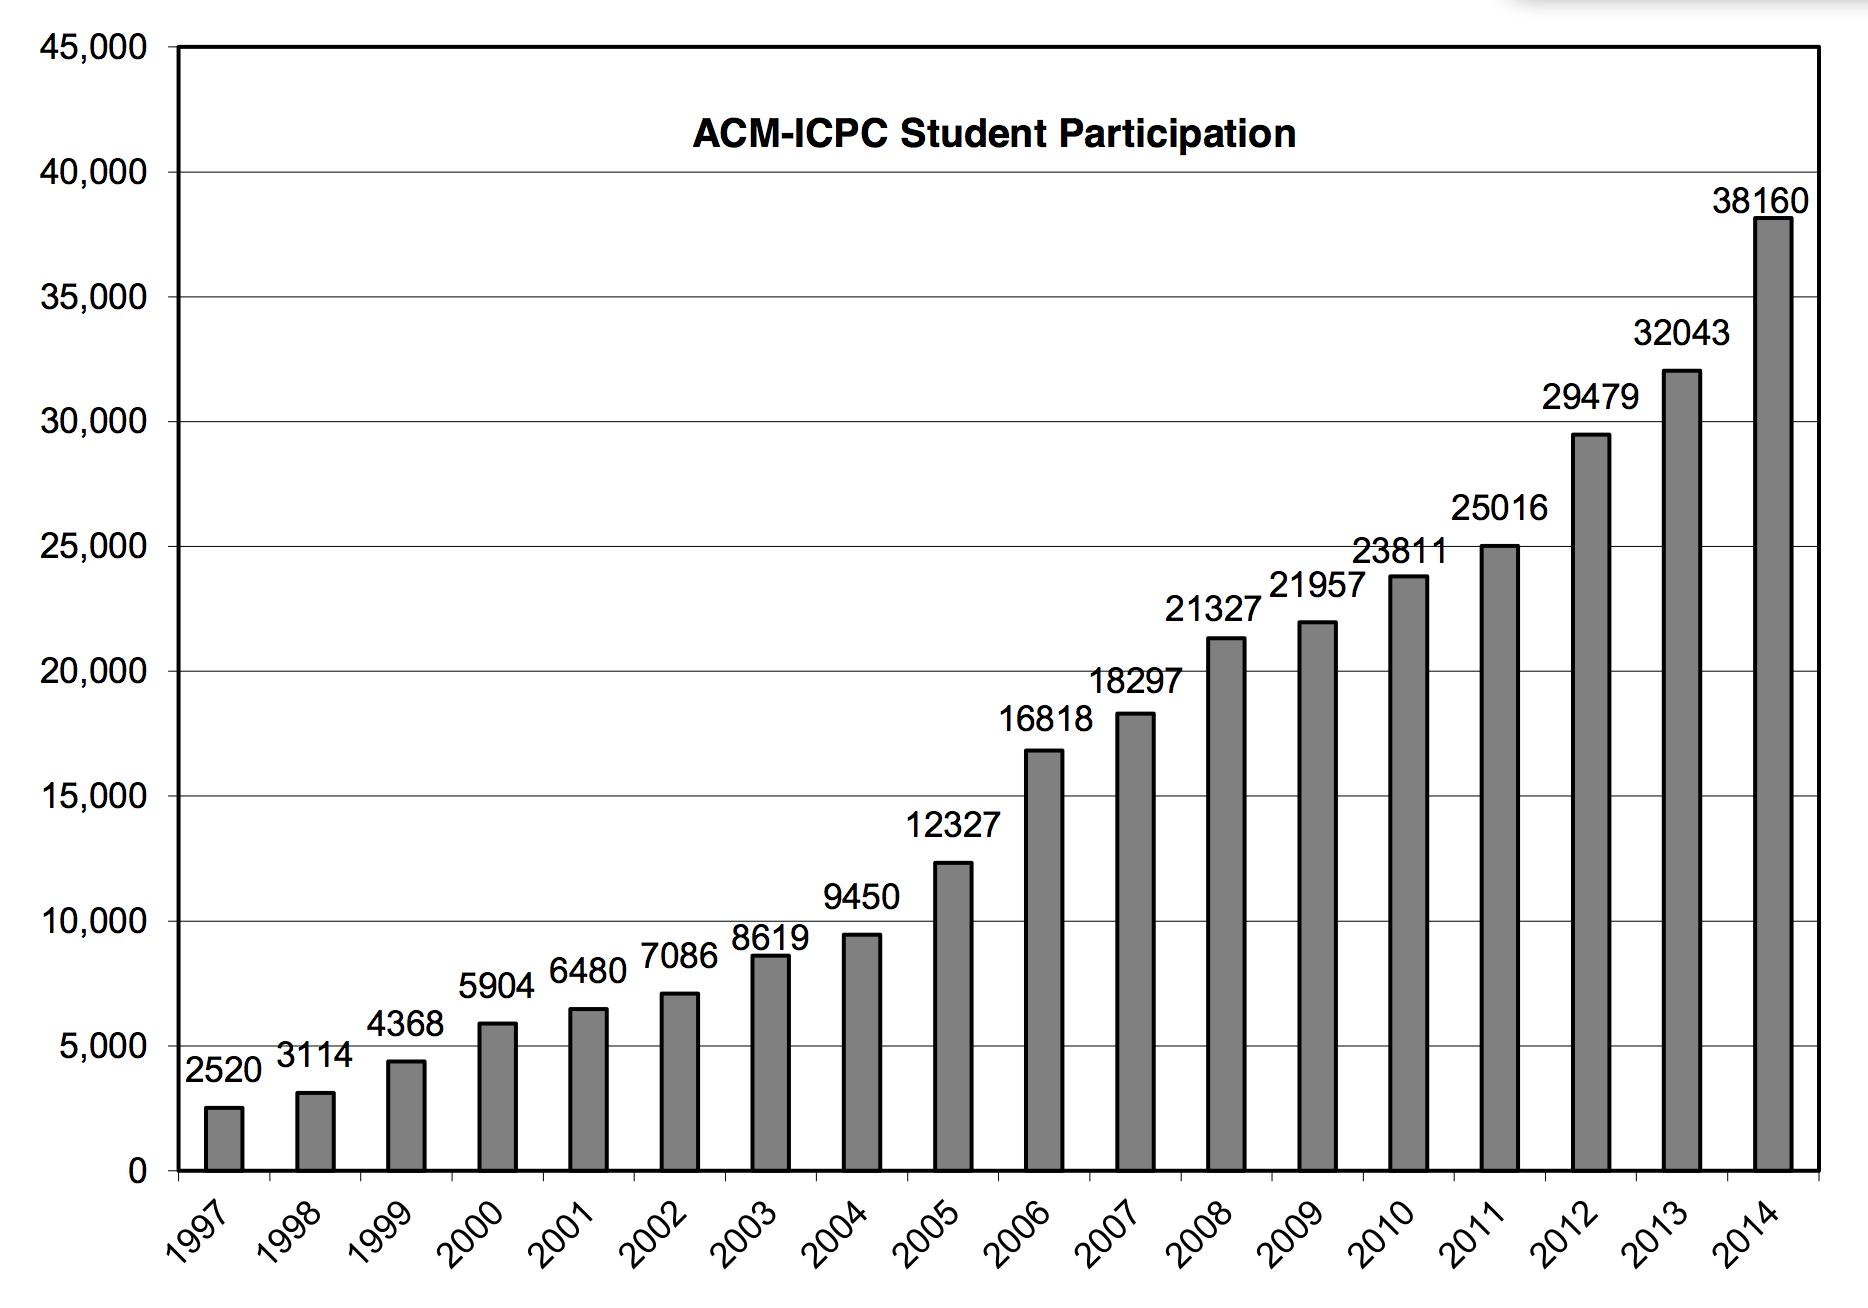
\includegraphics[width=0.4\linewidth]{grafico.png}
    \caption{Crescimento do n\'umero de participantes por ano.}
\end{figure}
}

\frame{
	\begin{center}
	\huge
	Obrigado!!
	\end{center}
}

\end{document}
